\documentclass[11pt,a4j,uplatex]{jsarticle}
\usepackage{ascmac}
\usepackage{amsmath}
\usepackage[dvipdfmx]{graphicx}
\usepackage{upgreek}
\usepackage{cases}%連立方程式
\usepackage{bm}%ベクトル表記\bm{A}
\usepackage{bigdelim,multirow}

\newsavebox{\circlebox}
\savebox{\circlebox}{\fontencoding{OMS}\selectfont\Large\char13}
\newlength{\circleboxwdht}
\newcommand{\centercircle}[1]{%
  \setlength{\circleboxwdht}{\wd\circlebox}%
  \addtolength{\circleboxwdht}{\dp\circlebox}%
  \raisebox{0.4\dp\circlebox}{%
    \parbox[][\circleboxwdht][c]{\wd\circlebox}{\centering#1}}%
  \llap{\usebox{\circlebox}}%
}	%丸数字(文字)環境。\centercircle{入れたい文字} で丸文字を表示する。


\title{Semiconductor Optics 和訳}
\author{3.2,3.3}

\makeatletter%図番号定義
%\renewcommand{\figurename}{Firuge}%図表記をFigure *.*へ
\renewcommand{\thefigure}{\thesection.\arabic{figure}}%図 章番号.図番号
\makeatletter

\begin{document}
\if0
\maketitle %タイトル

\thispagestyle{empty}%このページにはページ番号を入れない.
\clearpage
\addtocounter{page}{-1}


\tableofcontents %目次

\thispagestyle{empty}%このページにはページ番号を入れない
\clearpage
\addtocounter{page}{-1}

%\listoffigures%図目次。確認用。後で消す
\fi
\setcounter{section}{3}
\setcounter{subsection}{1}
\setcounter{figure}{15}
\newpage
\subsection{微視的側面}
先行した単元とは対照的に、今回は、微視的観点からの、光と物質の間の基本的な相互作用過程を与える。
光と物質の間の相互作用のために、摂動や、弱い結合をここで用いる。これは、ほとんどの場合、ガスのような希薄な系で十分である。固体においては、強い結合が必要不可である(それはポラリトンの概念を導く。チャプター5にて紹介する)。セクション3.2.1では、吸収、自然放出、誘導放出と名付けられている、光と物質の間の基本的な対応過程について述べる。セクション3.2.2では、摂動理論の枠組みの中の、線形の光学特性の扱いを説明する。それらのトピックは多くの本にて扱われているので([81M1,90K1,96Y1]のチャプター1や、[55S1,71F1,73H1,76H1,92M1]のチャプター2等を参照。)、ここでは詳細を述べる必要はない。
\subsubsection{吸収、自然放出、誘導放出と仮想励起}
簡単のため、図(3.16)のような、一定の数の2準位"原子"を仮定する。すべての原子は、基底状態か励起状態のどちらかである1つの電子を持っている。後々この2準位系を、半導体におけるバンドにまで拡大するが、基本的な対応過程は同じである。
\begin{figure}[b]
  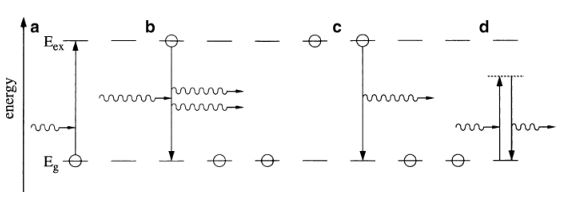
\includegraphics[clip]{4way.jpeg}
  \caption{光学応答概略図(a:吸収、b:誘導放出、c:自然放出、d:仮想励起子).}
\end{figure}
図(3.16a)では、入射した光子が、基底状態の原子に衝突している。一定の確率で光子は消滅して、電子は励起状態へ遷移するのに十分なエネルギーを受け取る。エネルギー保存則から、光子は
\begin{equation}
  \hbar\omega=E_{\mathrm{ex}}-E_{\mathrm{g}}\tag{3.36}
\end{equation}
の関係を満たす必要がある。ここで、右辺は励起状態と基底状態のエネルギー差である。もし光子のエネルギーがほかの形に変換されたら、その過程を吸収と呼ぶ。そして、電子が散乱過程を受けたら、コヒーレンスを破壊するか、電子的な偏光のより正確なコヒーレンスとなって入射光場の遷移につなげられる。これについては、チャプター23を見ること。電子はやがて基底状態に戻り、例えば格子振動や熱、入射光とコヒーレントでない光となってエネルギーを失う。前者を非放射遷移、後者を蛍光共鳴と呼ぶ。

もし入射光が、励起状態の電子を伴う原子に衝突したとき、一定の確率で、励起状態から基底状態への電子の遷移を誘発する。この過程においてでは、2つ目の光子は入射光と同じ運動量、エネルギー、偏光状態、位相で作られる。この過程は誘導放出あるいは刺激放出と呼ばれる。この過程は光場を増幅する。したがって、これはすべてのレーザー(Light Amplification by Stimulated Emission of Radiation:放射線の誘導放出による光の増幅)の基本の機構となる。吸収と誘導放出は密接な関係を持つ現象である(図(3.16b))。

励起状態の電子は一定の確率で光子を放出する(図(3.16c))か、フォノンや衝突を通してエネルギーを失うか、のどちらかを行うことで基底状態に戻る。この章では、前者のメカニズムが重要である。前者は自然放出あるいは自然放射性再結合と呼ばれ、後者は非放射性再結合としても知られる。自然放出はほかの考え方で理解することもできる。セクション2.5で、式(2.54)に関連して、光子は調和振動に似ていて、結果としてゼロ点エネルギーを持つことを見た。このゼロ点エネルギーはすべての光子のモードに存在する。ゼロ点エネルギーは、調和振動はゼロ点以下のエネルギーを持てないことから、吸収されない。しかし、これは図(3.16b)に関連して論じたように、遷移を誘発することができる。そのため、自然放出は電磁場のゼロ点振動(これは、電磁場の真空ゆらぎまたはゼロ点ゆらぎとも呼ばれる)によって誘発されたとみなすことができる。

最後の過程は仮想励起である。この現象を理解することはしばしば学生たちにとっていくつかの問題を起こす。そのため、このトピックはゆっくり進行し、図(3.16d)とともに、様々な観点、文脈からの説明を試みる。仮想励起は、励起状態と波動関数がおなじで、固有エネルギーが少しだけ違う状態が作られたことを意味する。この過程は、空間座標と運動量座標で書かれた量子力学の不確定性原理を通して可能となる。
\begin{equation}
  \Delta x_i\Delta p_i\geq h \,(i=1,2,3)\tag{3.37a}
\end{equation}
同じような関係が、エネルギーと時間の間にも存在する。
\begin{equation}
  \Delta E\Delta t\approx\hbar\tag{3.37b}
\end{equation}
ここで、式(3.37b)が必要になる。この式は、上記の条件を満たす最大時間$\Delta t$まで、$\Delta E$だけエネルギー保存則が破壊できることが可能である、と言っている。%なんのこっちゃ

言い換えると、$\Delta E$の確かな精度でエネルギーを定義したいとき、その状態は最低$\Delta t$の間存在しなくてはならない。式(3.37b)はまた、単純な古典的な(音波のような)波の理論で有効で、フーリエ変換としてよく知られている。$\Delta t$の時間だけ続く中心振動数$\omega$の調和振動は式(3.37c)で与えられるスペクトル幅$\Delta \omega$をもっている。
\begin{equation}
  \Delta\omega\Delta t\geq1\tag{3.37c}
\end{equation}
式(3.37b)と式(3.37c)の間には、次のような関係がある。
\begin{equation}
  E=\hbar\omega\tag{3.37d}
\end{equation}
これは式(3.37a)で使われている同様の一連の議論でも述べるべきである。もし、エネルギー$\hbar\omega'$を持った光子が原子に入射された時、最大$\Delta t$のあいだ、電子を励起することができる。$\Delta t$は、式(3.37b)か(3.38)によって与えられる。
\begin{equation}
  \Delta t\approx\hbar[\left|(E_{\mathrm{ex}}-E_{\mathrm{g}})-\hbar\omega'\right|]^{-1}\tag{3.38}
\end{equation}

少なくとも$\Delta t$秒経過したとき、励起状態は崩壊する。崩壊の最も単純な方法は、仮想励起を引き起こしたのと同じ光子を放出することである。この"新しい"光子は、エネルギーが$\Delta t$の間だけ原子に保持されているから、入射した光子に対して確かな位相差を持つ。その結果、真空よりも低い位相速度で、原子の集合を電磁波が伝搬する。同じ効果が、屈折率$n(\omega)$を用いて現象論的に述べられている(式(2.15)、(2.41))。そのため、量子力学において、どうやって$n(\omega)$が理解され、計算されたかについて、ヒントを得ることができる。式(3.38)において共振状態に近づいた時、明らかに$\Delta t$は増加し、結果として物質中の波の伝搬が真空中の波の伝搬から大きく逸れる。セクション4.3でみられるように、これは確かにそうである。

もし仮想励起状態がエネルギー$\hbar\omega'$の光子を、入射してきた光子とは違う方向に放出したとき、式(3.26)で議論したように、散乱過程を得る。もしエネルギー$\hbar\omega'$の光子が共振エネルギーに近い場合、この散乱過程は、すでに上で言及したように、蛍光共鳴として知られる。

この散乱に関連して、どのように、クリアなあるいは透明な媒体中を光が伝搬するのか?その答えは、高密度の物質中で、それが白熱灯やレーザー、その他どの光源からの光なのかに依らずに、光のコヒーレントな体積の中に、散乱原子や散乱中心を持っていることである。その結果、すべての散乱波は、位相の異なる光を見つけ、最終的に破壊された散乱の中にいる。すべての散乱波が簡潔に干渉する唯一の方法は、常に伝搬波であることである。青い空の説明での(セクション3.1.5で得たように)、散乱中心の直径が散乱放射線の波長に比べ小さいという条件のほかに、別の結合、すなわちガス分子のような、2,3の散乱中心しかない状態密度ゆらぎや太陽光のコヒーレント体積のほかの不均一性によって、互いに破壊的な散乱波の干渉は完成していない。空間的や時間的なコヒーレンスの詳細な説明については、[07M1,07S1]のチャプター1や[73C1,93S1]のチャプター2等を見ること。%さっぱりわからん

もし仮想的な励起状態が、光子の誘導放出とフォノンの生成消滅(たとえば、セクション11.1のような格子振動の量子)の下で消えたら、放出された光子のエネルギー$\hbar\omega_R$は式(3.39)に従う。
\begin{equation}
  \hbar\omega_{\mathrm{R}}=\hbar\omega'\pm\hbar\Omega_{\mathrm{phonon}}\tag{3.39}
\end{equation}
この現象は光学フォノンの場合はラマン散乱と呼ばれ、音響フォノンの場合はブリルアン散乱と呼ばれる。"-"の符号はストークス放出、"+"の記号は反ストークス放出を与える。同じような過程が、1つ以上のフォノンや、半導体中の電子やスピンシステムの中での励起子でも可能である。仮想励起を含むいくつかの現象の簡単な概念によると、このメカニズムが物質の光学特性にとって重要なのは明らかである。それゆえ、これを、他の観点や、古典的でアナログによく知られている仮想励起状態についての概念で試したい。この類推は、チャプター4で使われる誘電関数の計算におけるいくつかの理由も与えてくれる。

量子力学における仮想励起は、古典的な駆動振動や強制振動にも対応している。もし、固有振動数$\omega_0$(量子力学においてのエネルギー差$(E_{\mathrm{ex}}-E_{\mathrm{g}}$)に対応している)の振動子があり、もしこれを外部の振動$\omega$で励起させたら、$\omega_0$での短い過渡特性の減の後、$\omega$で振動する。振動の特性による$\left|\omega-\omega_0\right|$の離調の減少(例えば減衰)を伴って、これらの安定した振幅は増加する。これらの古典的な振動の振幅の増加は、仮想励起の図の、式(3.39)の$\Delta t$に対応し、それの適格性は、$\omega_0$の共振の近傍において、$\epsilon(\omega)$や$\tilde{n}(\omega)$が、真空における値$\epsilon=\tilde{n}=1$から強く逸脱していることから理解できる。この概念はチャプター4で詳細に述べる。

しかし、そうする前に、図(3.16)にみられる複数の種類の遷移やその他が、摂動理論の量子力学においてどのようにして、定量的に扱われるのかを実演する。

\newpage
\subsubsection{光と物質の線形相互作用の摂動的取り扱い}
このセクションでは、まず摂動項を詳しく述べる系のハミルトニアンについて説明する。次に摂動がどうやって様々な固有状態の間の遷移を引き起こすのか、の概説をする。最後に、これら二つのことを、吸収と誘導放出、自然放出についての論理的な説明の理解とともに結びつける。

図(3.16)の2つの準位の原子(あるいは半導体のバンド図)の電子状態と放射場、二つのこれらの系の相互作用から成っているすべての系のハミルトニアンは式(3.40)のように書かれる。

\begin{equation}
  H=H_{\mathrm{el}}+H_{\mathrm{rad}}+H_{\mathrm{interac}}\tag{3.40}
\end{equation}
セクション2.5の2つの量子化概念の図で、$H_{\mathrm{interac}}$は、光子と基底状態の電子の消滅と図(3.16a)で見られる過程の励起状態の電子の生成の項を含む。その項は遷移行列要素を含む因子で重みづけされている。

すべてのハミルトニアンの正確な解法は、線形光学の分野のポラリトン(チャプター5)の概念を導き、セクション20.1から20.4に例が見られる非線形光学における放射の存在によって紹介される電子の状態の変化について特に述べる。

現在の目的のために、小さな摂動のような放射場において使われ、そしてそれを扱う手法を用いる。つまり、電磁場の存在の中でのものとあまり変わらない、$H_{\mathrm{el}}$の固有状態$\phi$と固有エネルギー$E_{\mathrm{n}}$を仮定する。また、$H_{\mathrm{rad}}$の固有状態は、セクション2.5で述べられた光子である。今使っている近似は放射の純古典的な扱いとして知られている。これは正準共役運動量$\bm{p}$を
\begin{equation}
  \bm{p}\to \bm{p}-e\bm{A}\tag{3.32}
\end{equation}
としてハミルトン関数に含む($\bm{A}$はベクトルポテンシャル(式(2.48)))。

もし$\bm{p}$を、演算子を用いて
\begin{equation}
  \bm{p}=\frac{\hbar}{i}\nabla\tag{3.42}
\end{equation}
のように入れ替えたら、単一粒子のハミルトニアンは、静電ポテンシャル$V(\bm{r})$を用いて
\begin{equation}
  H=\frac{1}{2m}(\frac{\hbar}{\mathrm{i}}\nabla-e\bm{A})^2+V(\bm{r})\tag{3.43}
\end{equation}
と書ける。クーロンゲージ(式(2.49)を用いて、式(3.43)を変形して
  \begin{align}
    H&=-\frac{\hbar^2}{2m}\nabla^2+V(\bm{r})-\frac{e}{m}\bm{A}\frac{\hbar}{\mathrm{i}}\nabla+\frac{e^2}{2m}\bm{A}^2\tag{3.44}\\
    H&=H_{el}-\frac{e}{m}\bm{A}\frac{\hbar}{\mathrm{i}}\nabla+\frac{e^2}{2m}\bm{A}^2\tag{3.45}\\
    H&=H_{el}+H^{(1)}+H^{(2)}\tag{3.46}
  \end{align}
式(3.46)には、$H^{(1)}$と$H^{(2)}$の2つの摂動項がある。Aを仮定して、光強度が十分小さいとき(ただし、線形光学系では光強度は定義によって小さい)、$H^{(1)}$は1次の摂動項、$H^{(2)}$は小さい2次の摂動項である。その結果、$H^{(1)}$は1次摂動理論の中で使われなければならない。2次の近似においては、2次摂動理論における$H^{(1)}$と、1次摂動理論における$H^{(2)}$等を使わなければならない。後者の側面はチャプター19で述べる。%なにこれ?

初期状態$i$(図(3.16)におけるg)から別の状態$j$(図(3.16)におけるex)への遷移レート$w_{ij}$にフェルミの黄金律を適用することによって、時間依存のシュレディンガー方程式
\begin{equation}
  H\psi=\mathrm{i}\hbar\frac{\partial\psi}{\partial t}\tag{3.47a}
\end{equation}
が使え、定常状態$H=H_0$の時の解は
\begin{equation}
  \psi_{\mathrm{n}}(\bm{r},t)=\phi_{n}(\bm{r})\mathrm{e}^{-\mathrm{i}(E_{\mathrm{n}}/\hbar)t}\tag{3.47b}
\end{equation}
である。摂動$H^{(1)}$の存在を解くために、式(3.48)を作る。
\begin{equation}
  \psi_{\mathrm{n}}(\bm{r},t)=\sum_{\mathrm{n}}a_{\mathrm{n}}(t)\phi_{\mathrm{n}}(\bm{r})\mathrm{e}^{-\mathrm{i}(E_{\mathrm{n}}/\hbar)t}\tag{3.48}
\end{equation}
摂動が$t=0$の時に始まると仮定する。系が状態$i$である前は
\begin{equation}
\left.
\begin{array}{ccc}
a_{\mathrm{i}}(t)=1\\
a_{\mathrm{n\not=i}}(t)=0
\end{array}
\right\}  \mathrm{for}\:t\leq0\tag{3.49}
\end{equation}
である。$t>0$のとき$a_{\mathrm{n\not=i}}(t)$は増加し、この状態では、フェルミの黄金律の遷移レート$w_{ij}$は
\begin{equation}
  w_{ij}=\frac{2\pi}{\hbar}\left|H_{ij}^{(1)}\right|^2D(E)\tag{3.50a}
\end{equation}
となる。ここで$D(E)$は、該当するなら、運動量保存則によって修正された最終状態の密度である。$H_{ij}^{(1)}$は式(3.50b)によって与えられる遷移行列要素である。
\begin{equation}
  H_{ij}^{(1)}=\int\psi_j^*(\bm{r})H^{(1)}\psi_j(\bm{r})\mathrm{d}\tau=:\langle\psi_j\left|H^{(1)}\right|\psi_i\rangle\tag{3.50b}
\end{equation}
縮退していない2準位系において、$D(E)$は原子1つにつき単に1つである。正方遷移行列要素$\left|H_{ij}\right|^2$は遷移確率として知られている。後程、記述を簡単にするために、$2\pi/\hbar$項のような、$\left|H_{ij}\right|^2$に組み込まれた定数項を仮定する。遷移確率は、1次摂動の場合は式(3.50)の、2次摂動の場合は式(3.51)のそれぞれの正方遷移行列の要素による係数とは別に与えられえる。

遷移レート$w_{ij}$は、$H^{(1)}$の振幅の2乗(すなわち、$\left|A_0\right|^2\sim I$($I$はここでは光強度))が掛けられた遷移確率と比例関係にある。すなわち、すでに述べたように、単位領域および単位時間ごとのエネルギー流速である。%なにがなんだか

式(3.50b)の1次摂動項が消滅したら、2次の寄与で述べたことによって、
\begin{equation}
  w_{ij}^{(2)}=\frac{2\pi}{\hbar}\left|\sum_{k\not=i.j}\frac{H_{jk}^{(1)}H_{ki}^{(1)}}{E_i-E_k}+H_{ij}^{(2)}\right|^2D(E)\tag{3.51}
\end{equation}
と導ける。式(3.50)によって1次のモーメントを制限し、式(3.45)の摂動の詳細の中で、$H_{ij}^{(1)}$の項について議論する。ベクトルポテンシャルを
\begin{equation}
  \bm{A}=\bm{A}_{\mathrm{0}}e^{i(\bm{kr}-\omega t)}\tag{3.52a}
\end{equation}
とすると、遷移レート$w_{ij}$は、式(3.50)の吸収過程のように、
\begin{equation}\tag{3.52b}
  \begin{split}
    w_{\mathrm{g\to ex}}&=\frac{2\pi}{\hbar}\left|\frac{-e\hbar}{\mathrm{i}m}A_0\cdot \int\phi_{\mathrm{ex}}^*(\bm{r})\mathrm{e}^{\mathrm{i}(E_\mathrm{ex}/\hbar)t}\bm{e}_A\mathrm{e}^{\mathrm{i}(\bm{kr}-\omega t)}\nabla\phi_{\mathrm{g}}(\bm{r})\mathrm{e}^{-\mathrm{i}(E_\mathrm{g}/\hbar)t}\mathrm{d}\tau\right|^2D(E_{g}+\hbar\omega)\\
    &\propto\left|A_0\langle\phi_{\mathrm{ex}}|H^{(1)}|\phi_{\mathrm{g}}\rangle\right|^2D(E_{g}+\hbar\omega)\\
    &=:A_0^2\left|H_{\mathrm{eg}}^{(1)}\right|^2D(E_{g}+\hbar\omega)
  \end{split}
\end{equation}
となる。ここで、$\bm{e}_{\mathrm{A}}$は$\bm{A}$方向の単位ベクトルである。(3.52)は、積分の省略形としても一般に使われる。重要な遷移レートは、時間依存の指数関数が消滅するときに発生し、あるいは数学的に
\begin{equation}
  E_{\mathrm{ex}}-E_{\mathrm{g}}-\hbar\omega=0\tag{3.53a}
\end{equation}
を満たすときのみ発生する。これは、エネルギー保存則である。もし$\phi_i$や$H^{(1)}$が平面波の性質を持っていて、波数ベクトル$\bm{k}$によって記述されるとき、この式は$\bm{k}$に対応する似たような結果をもたらす。
\begin{equation}
  \hbar\bm{k}_{\mathrm{ex}}-\hbar\bm{k}_{\mathrm{g}}-\hbar\bm{k}=0\tag{3.53b}
\end{equation}
これは、ここで議論されている2準位系の原子だけでなく、結晶の半導体の固有状態にも、ほとんどの場合成り立つ。
遷移レートは$A_0^2$に、そして特定のモードにおいて、光強度$I=\langle S\rangle$あるいは光子密度$N_{\mathrm{ph}}(\omega)$に比例する。
\begin{equation}
  w_{ij}\propto A_0^2\left|H_{\mathrm{eg}}^{(1)}\right|^2\propto I\left|H_{\mathrm{eg}}^{(1)}\right|\propto N_{\mathrm{ph}}\left|H_{\mathrm{eg}}^{(1)}\right|\tag{3.54}
\end{equation}
固有関数が正規直交集合の形をとること、$H^{(1)}$がハミルトニアンに追随すること、あるいは$H^{(1)}$によって誘発された、$i\to j$や$j\to i$の状態遷移の微視的可逆性の議論によって部分積分を使うことにより、次の式を得る。
\begin{equation}
  \left|\int\phi_j^*H^{(1)}\phi_i\mathrm{d}\tau\right|^2=\left|\int\phi_i^*H^{(1)}\phi_j\mathrm{d}\tau\right|^2\tag{3.55}
\end{equation}
誘導放出や吸収の確率は同じで、上の状態と下の状態の原子の数を含む因子の確率が違うだけである。この事実はアインシュタイン係数の関係の基礎である。これについては、セクション3.3の課題10を見ること。自然放出はゼロ点から刺激された放出として扱われるべきである。この側面に戻ってみる。最初に、交換演算子$H^{(1)}$は双極子近似と呼ばれるために単純化されるべきである。

原子半径($r\simeq0.1 nm$)や液中における原子間距離($a\simeq0.3 nm$)は可視域の波長($\lambda\simeq500 nm$)に比べ小さいことに注意。それゆえ、事実上、単原子や隣接原子との間での電磁放射の位相の変化はない。したがって、式(3.52)の$\mathrm{e}^{\mathrm{i}\bm{kr}}$の項をべき級数に拡張することができ、定数項の後に止まる。
\begin{equation}
  \mathrm{e}^{\mathrm{i}\bm{kr}}=1+\frac{\mathrm{i}\bm{kr}}{1!}+\frac{{(\mathrm{i}\bm{kr}})^2}{2!}+...\simeq1\tag{3.56}
\end{equation}
これは双極子近似の最初の段階である。その意味は、光子の運動量$\hbar\bm{k}$を無視することである。

行列要素$H_{ij}^{(1)}$は運動量演算子$\bm{p}=\frac{\hbar}{i}\bm{\nabla}$を含む。
\begin{equation}
  H_{ij}^{(1)}\sim\langle\phi_{\mathrm{i}}\left|\bm{p}\right|\phi_{\mathrm{i}}\rangle=:\langle\bm{p}_{\mathrm{i,j}}\rangle
  \nonumber
\end{equation}
準古典的関係
\begin{equation}
  \frac{\hbar}{i}\bm{\nabla}=p=m\dot{\bm{r}}\tag{3.57}
\end{equation}
といくつかの議論の妥当性によって、
\begin{equation}
  \int\phi_j^*\frac{\hbar}{\mathrm{i}}\bm{\nabla}\phi_{\mathrm{i}}\mathrm{d}\tau=m\frac{\mathrm{i}}{\hbar}(E_i-E_j)\int\phi_j^*\bm{r}\phi_{\mathrm{i}}\mathrm{d}\tau=m\omega\int\phi_j^*\bm{r}\phi_{\mathrm{i}}\mathrm{d}\tau\tag{3.58}
\end{equation}
がわかる。この関係性の詳しい導出のために、波動関数の知識が要求される(詳細はチャプター2の[55S1,85G1,92M1]等)。

この、いわゆる双極子近似(式(3.56))において遷移レートは
\begin{equation}
  w_{ij}\sim I\omega^2\left|e_A\langle e\bm{r}_{ij}\rangle\right|^2D(E)=I\omega^2\left|H_{ij}^D\right|^2D(E)\tag{3.59}
\end{equation}
で与えられることに注意。ここで、$e_{\bm{A}}$は$\bm{A}$方向の単位ベクトルで、$\left|H_{ij}^D\right|$は、場の振幅の2乗が光場$I$の強度の中ですでに表れているように、双極子モーメント$e\bm{r}$の期待値の2乗である。

混乱を避けるために、$\left|H_{ij}^D\right|$が双極子モーメント演算子のみを含むのに対し、$\left|H_{ij}^{(1)}\right|$は$\bm{A}$や$\bm{E}$の強度を含み、エネルギーの次元を持っていることに注意する。

この結果は、電磁場$\bm{E}=\dot{\bm{A}}$においての双極子$e\bm{r}$のエネルギーが
\begin{equation}
  e\bm{r}\cdot\bm{E}=H^{(1)}\tag{3.60}
\end{equation}
で与えられることを覚えていれば、式(3.50)から式(3.59)を直接計算するという直感的な方法で得ることもできる。
あるいはこれは、チャプター1の[07M1]の式(3.57)での、摂動項$-e\bm{pA}/m$を$e\bm{rE}$と取り換えることができるという似た議論にみられる。式(3.45)の1次の摂動項と(3.60)を比較する。%えらいこっちゃ

今後、$\left|H_{ij}^D\right|$を双極子遷移レートと呼び、演算子$e\bm{r}$を双極子演算子$\left|H^D\right|$とする。

この結果は、$\bm{A}$に、クーロンゲージ$(\bm{\nabla\cdot A}=0)$ではない適したゲージ$\bm{A}'=\bm{A}+\nabla\chi$および$\Phi=\Phi-\dot\chi$($\chi$は既存の2次導関数をもつスカラー場)を使うことから導かれる。$A'$は$A$のような同一の電場及び磁場に起因する。$\chi(\bm{r},t)=i\omega^{-1}\bm{rE}=i\omega^{-1}\bm{r}\bm{E}_0exp[i(\bm{kr}-\omega t)]$の選択は式(3.60)の$H^{(1)}$に起因する。

式(3.44)や(3.51)、(3.56)の高次項における遷移は四重極や五重極、それ以上の極に対応する。

このセクションを終えるために、図(3.16(a-c))の正味の遷移レートを計算する。

セクション2.6で状態密度の計算に使われた考え方のような一つのモードの光子密度$N_{\mathrm{ph}}$を、つまりすべての光子が同じ波数ベクトル$\bm{k}$や偏光状態$e_{\mathrm{A}}$、エネルギー$\hbar\omega$を持っているときを仮定する。

さらに、$\hbar\omega$は式(3.54)のエネルギー保存則を満たしている。同一の二準位原子密度は$N_{\mathrm{A}}$である。ここで、$\alpha_{\mathrm{g}}$は基底状態の割合で、それに対応して$(1-\alpha_{\mathrm{g}})$は励起状態の割合である。$N_{\mathrm{ph}}$の正味の時間変化率は、式(3.54)と(3.59)を用いて
\begin{equation}
  \frac{\partial N_{\mathrm{ph}}}{\partial t}=-N_{\mathrm{A}}\alpha_{\mathrm{g}}N_{\mathrm{ph}}\left|H_{\mathrm{g\to e}}^D\right|^2+N_{\mathrm{A}}(1-\alpha_{\mathrm{g}})(1+N_{\mathrm{ph}})\left|H_{\mathrm{g\to e}}^D\right|^2\tag{3.61}
\end{equation}
で与えられる。右辺第一項は光子の吸収、第二項は因子$(1+N_{\mathrm{ph}})$を用いて、誘導放出及び自然放出について述べている。

式(3.55)から
\begin{equation}
  \left|H_{\mathrm{g\to e}}^D\right|^2=\left|H_{\mathrm{e\to g}}^D\right|^2=\left|H^D\right|^2\tag{3.62}
\end{equation}
とでき、それゆえ
\begin{equation}
  \frac{1}{\left|H^D\right|^2}\frac{\partial N_{\mathrm{ph}}}{\partial t}=N_{\mathrm{ph}}\cdot N_{\mathrm{A}}(1-2\alpha_{\mathrm{g}})+N_{\mathrm{A}}(1-\alpha_{\mathrm{g}})\tag{3.63}
\end{equation}
となる。右辺第一項は$N_{\mathrm{ph}}$の線形に依存し、吸収と誘導放出の正味の確率について述べている。第二項は$N_{\mathrm{ph}}$に依存しない自然放出について述べている。

$\alpha_{\mathrm{g}}>1/2$(吸収係数$\alpha(\omega)>0$あるいは$\partial N_{\mathrm{ph}}/\partial t<0$)のとき正味の吸収があり、$\alpha_{\mathrm{g}}<1/2$のとき増幅あるいは光利得がある。すなわち、利得のためには、半分以上の原子が上の状態にいなければならない。この状況は熱平衡には届かず、励起強度の適切な供給の影響下にある。通常、一つかそれ以上の追加のエネルギー準位が要求される(三準位、四準位レーザー)。この事実は次のような議論で簡単に明らかにされる。すべての原子が基底状態にある状態(すなわち、$\alpha_{\mathrm{g}}|_{t=0}$\,=1)から考える。$t>0$において、式(3.52a)を満たすような波長$\omega$の光子を系に送ったとき、吸収は初めに、$\alpha(\omega)$を用いて
\begin{equation}
  -\alpha(\omega)\sim N_{\mathrm{A}}(1-2\alpha_{\mathrm{g}})\tag{3.64}
\end{equation}
と与えられる。時間と励起光強度を増加させていくと、$\alpha_{\mathrm{g}}$が減少するため$\alpha(\omega)$は減少する。$\alpha_{\mathrm{g}}=1/2$のコヒーレントでない原子の励起分布によって、吸収は消え、物質は光を透過させる。これは、励起の(疑似)定常状態において、これ以上の励起では$\alpha_{\mathrm{g}}>1/2$に届かないことを意味する。チャプター21-23で、セクション2.6で紹介した、適切な統計を用いた上記の考察について再検討する。チャプター23や27で、位相ずれの過程がないとき、あるいは位相ずれの時間よりも十分激しいパルスを用いた時、周期的に、基底状態から完全に反転させた状態$(\alpha_{\mathrm{g}}=0)$に系を動かし、再び元に戻ることが可能になる、ということについて見る。この過程をラビ振動と呼ぶ。
\end{document}
